\subsection{Registro de un usuario}

En cuanto a este diagrama, se representa la operación de registro de un usuario con rol de administrador. Si todo ocurre según lo esperado, el usuario deberá recibir una confirmación de que el usuario se registró correctamente.

\begin{figure}[H]
\centerline{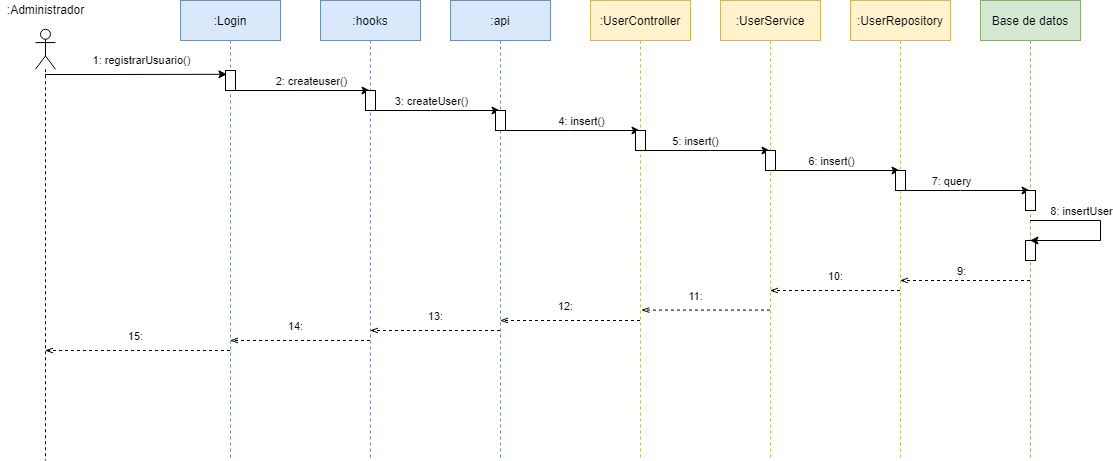
\includegraphics[width=15cm]{figuras/diseño/RegistroUsuario.png}}
\caption{Diagrama de secuencia 01. Registro de un usuario.}
\label{enlaceDRegistro}
\end{figure}

\begin{enumerate}
    \item El usuario pincha en el botón de registro de usuarios.
    \item Este método invoca el método createUser() del archivo contenido en hooks().
    \item Se invoca al método createUser() de la carpeta api.
    \item Se hace un llamamiento mediante una solicitud HTTP al servidor. En concreto, la función insert() de UserController, pues se hace un POST.
    \item Se invoca al servicio insert() de UserService.
    \item Se invoca la operación insert del repositorio UserRepository.
    \item Se invoca la operación de guardado en la base de datos de MongoDB.
    \item Se almacena el usuario en la base de datos.
    \item Se procede a devolver la respuesta al usuario desde este paso, realizando el proceso inverso. El usuario recibirá un mensaje de que la operación fue satisfactoria.
\end{enumerate}